\documentclass[11pt]{article}

\textwidth=6.05in
\oddsidemargin=0.4in
\evensidemargin=0.4in
\topmargin=-0.3in
\footskip=0.8in
\parindent=0.0cm
\parskip=0.3cm
\textheight=8in
%%% \renewcommand{\baselinestretch}{1.21}

\newcommand{\mynote}[1]{\begin{center}\fbox{\parbox{5in}{#1}}\end{center}}
\newcommand{\commentout}[1]{}

\usepackage{graphicx}

\begin{document}
\pagestyle{empty}

\def \handout#1#2
{\vspace*{-0.5cm}
\noindent
University of Pittsburgh\hfill \mbox{ }\\
CS 1571 Foundations of Artificial Intelligence \hfill Handout #1\\
\textbf{YOUR NAME HERE} \hfill #2
\hrule}


\def \problemset#1#2
{
\medskip
\begin{center}
        {\large \bf Problem assignment #1}\\
{\normalsize \em Due: #2}
\end{center}}

\handout{1}{January 16, 2024}
\problemset{1}{Friday, January 24, 2025}

Please note that homework assignments should be submitted to Canvas by midnight on the due date. This concerns both the reports and programs. The reports should be submitted in the pdf format. If you include any hand-made writings or drawings in the report please make sure they fit the page and are legible. The submissions (or their parts) that are not legible with a pdf reader will be left ungraded and receive zero score. Please submit one zipped archive containing all of your Python code. The end of this document specifies which files you need.


\subsection*{Problem 1. Map coloring problem}

Assume we want to solve the {\bf map coloring problem} in Figure 1. The goal is 
to color a map such that no countries on the map that share a border are assigned the same color. 
The number of colors is limited. In this assignment assume you have three different colors: 
Red, Green, and Blue. 
 
\begin{figure*}[!h]    
\begin{center}
	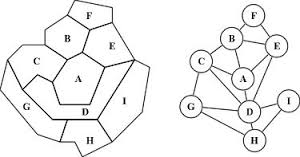
\includegraphics[width=7cm]{Graph_coloring_9_layout.jpg}
\caption{Map coloring problem. Left: spatial layout. Right: abstraction of the spatial layout where nodes correspond to countries and links to borders.}  
\end{center}
\end{figure*}

Part a. Formulate the map coloring problem as a (graph) search problem by defining its \textbf{initial state}, \textbf{successor function}, \textbf{goal test}, and \textbf{path cost}. To define the successor function, you should describe what actions are available and how they cause the state to change. 

\vspace{2cm} % replace with your answer

Part b. What is the search space size of the formulation in Part a? If the exact calculation of the search space size becomes hard, give a reasonable upper bound estimate. 

\vspace{2cm} % replace with your answer

Part c. Think of another possible formulation of the map coloring problem as the search problem. What is the search space size of this new formulation? Compare the first two formulations in terms of the search space size they define and determine which formulation appears more advantageous.

\vspace{2cm} % replace with your answer

Part d. Do you think you can solve the problem? If yes, please submit the solution. 

\vspace{2cm} % replace with your answer

\clearpage
\subsection*{Problem 2. Traveler problem}

Consider the following graph representing road connections
between different cities. Let S be the initial city and G the destination.
\begin{center}
	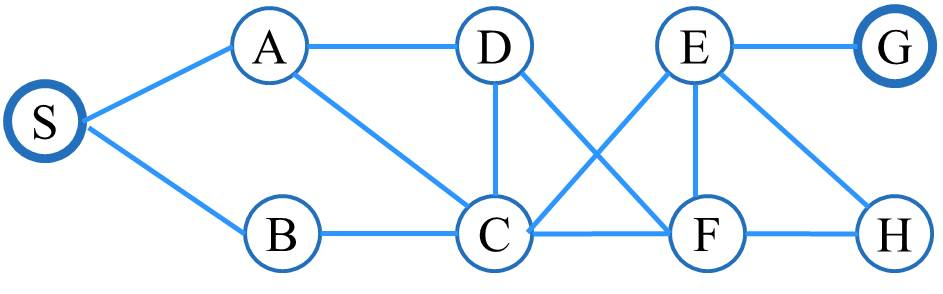
\includegraphics[width=0.8\textwidth]{./search_map_2.jpg}
\end{center}

Part a. Show how the breadth-first-search (with no state repeats checks) would search the
graph. That is, give an order (of first 10 nodes) in which the nodes could be {\em{expanded}}. Use alphabetical order to order equivalent choices. 


\begin{table}[h]
\begin{tabular}{|l|l|}
\hline
Expanded & Frontier \\ \hline
    S     & \{A,B\}        \\ \hline
         & \hspace{8cm}          \\ \hline
         &          \\ \hline
         &          \\ \hline
         &          \\ \hline
         &          \\ \hline
         &          \\ \hline
         &          \\ \hline
         &          \\ \hline
         &          \\ \hline
\end{tabular}
\end{table}

Part b. Show how the depth-first search \textit{with the elimination of cyclic state repeats} would search the graph by giving an order of first 10 {\em{expanded}} nodes. Use the alphabetical order to break the ties (i.e., equivalent node choices). A cyclic state repeat is one in which a node's child is already an ancestor of that node. 

\vspace{3cm}

Part c. Show how the breadth-first-search \textit{with elimination of cyclic repeats} only would search the graph. Give an order of first 10 expanded nodes.  Again, use the alphabetical order to break the ties (i.e., equivalent node choices).

\vspace{3cm}

Part d. Show how the breadth-first search that checks for \textit{all state repeats} would search the graph. Give an order of first 10 expanded nodes. ``All state repeats'' means that no single node will be expanded more than once.

Note: Please note it is possible the sequence of expanded nodes for some parts of the problem may be shorter than 10. In that case just list the nodes expanded before the goal state is reached.    

\vspace{3cm}

\subsection*{Problem 3. A problem-solving agent for the 8-puzzle problem.}

In this problem we will implement a number of uninformed search techniques and test them on the 8-puzzle problem. The rules for submitting the programs are described in Canvas. 

The 8-puzzle problem is described in the textbook (Russell and Norvig) on page 68. We have also studied the problem in lecture 2 (see lecture notes). The problem formulation of the 8-puzzle problem consists of: 
\begin{itemize}
\item States: different tile configurations
\item Operators: moves of an empty position
\item Initial configuration.
\item Goal configuration:\\
\begin{tabular}{|c|c|c|}
	\hline
      1 & 2 & 3\\
	\hline
      4 & 5 & 6\\
	\hline
      7 & 8 & 0\\
	\hline
\end{tabular}

where $0$ represents the empty (blank) tile. Note that the goal
configuration we consider is different from the configuration in
the textbook!
\item Solution (path) cost: the number of moves of the empty tile.
\end {itemize}

\subsubsection*{Part a. Run the plain breadth-first search algorithm.} 

To get you started in the assignment, you are given a python code implementation of the breadth-first search method for 8-puzzle. You can download the code using the assignment link in Canvas. 

The two files given are: 
\begin{itemize}
\item $Puzzle8.py$ that defines the Puzzle 8 problem, search tree nodes, a hash table, and 5 different game configurations to solve labeled as Example 1, ..., Example 5
\item $bfs.py$ that implements the basic breadth first search procedure and runs it in on 4 out of 5 initial game configurations.
\end{itemize} 
Once you run the code in $bfs.py$, you should see the solutions for four initial configurations. Three of the initial configurations are shown below: \\ 
\begin{tabular}{lcr}
\begin{tabular}{|c|c|c|}
	\multicolumn{3}{l}{Example 1:}\\
	\hline
	1 & 2 & 3\\
	\hline
	4 & 6 & 0\\
	\hline
	7 & 5 & 8\\
	\hline
\end{tabular}
&
\begin{tabular}{|c|c|c|}
	\multicolumn{3}{l}{Example 3:}\\
	\hline
	4 & 1 & 2\\
	\hline
	7 & 6 & 3\\
	\hline
	0 & 5 & 8\\
	\hline
\end{tabular}
&
\begin{tabular}{|c|c|c|}
	\multicolumn{3}{l}{Example 4:}\\
	\hline
	4 & 1 & 2\\
	\hline
	7 & 6 & 3\\
	\hline
	5 & 8 & 0\\
	\hline
\end{tabular}
\end{tabular}

Familiarize yourself with the python code given to you before proceeding to Part b. 

\subsubsection*{Part b. Breadth-first search statistics.}

Write a $breadth\_first\_search\_stats$ procedure that modifies the breadth first search procedure given to you in file $bfs.py$ such that it is able to collect and print the following statistics:
\begin{itemize}
\item the total number of nodes expanded;
\item the total number of nodes generated;
\item the maximum length of the queue structure;
\item the length of the solution path (number of moves)
\end{itemize}
The statistics should be printed after the example is solved and should be followed by the solution (move) sequence.  
Include the $breadth\_first\_search\_stats$ procedure in the $bfs\_stats.py$ file and use it to
execute it on the first four initial configurations similarly to $bfs.py$.

\subsubsection*{Part c. Breadth-first search with the elimination of cyclic state repeats.} 

The basic breadth-first search procedure 
does not check for and eliminate state repeats. In general, there are two strategies to eliminate state repeats:
\begin{itemize}
\item Elimination of cyclic state repeats: Do not expand the node if its state is the same as in one its ancestors in the search tree.
\item Elimination of all state repeats: Do not expand the node if its state has
been expanded before.
\end{itemize}
Note: Please see lecture notes for Lecture 3 on the elimination of state repeats. 

To implement the bfs with cycling check repeats you will need to write two pieces of code:
\begin{itemize}
\item function $check\_cyclic\_repeats(node)$ that takes a tree node and checks if the state linked to that node is also associated with one of its parent nodes in the search tree. The function should return true if the cyclic repeat indeed occurred. 
\item function $breadth\_first\_search\_cycles$ that modifies your code in Part b, such that prior to the node expansion it calls $check\_cyclic\_repeats(node)$ to check if we entered the cycle.   
\end{itemize}
Include the above two functions in the $bfs\_cycle.py$ file and run it on the same set of four examples we included in $bfs.py$ file. You may also try to solve the initial configuration in Example5. The function should collect and print the same statistics as in Part b.

\subsubsection*{Part d. Breadth-first search with the elimination of all state repeats.} 

Implement a $breadth\_first\_search\_repeats$ procedure that: (1) checks for and eliminates all state repeats, (2) collects and prints the same statistics as in Part b. 
Include the procedure in the $bfs\_repeats.py$ file and run it on all five test examples.  

To implement the elimination of all state repeats please use the hash table implemented in $Puzzle8.py$ file.  

{\bf Hint:} Similarly to the breadth first search with cyclic state repeats we recommend to check the node (its
state) for repeats just before the node is expanded, that is, after it
is extracted from the queue. Note that you do not have to check for cyclic
repeats since the all repeats test subsumes the cyclic repeats test. 

\subsubsection*{Part e. Analysis of the results}

Analyze the performance of all three bfs methods (parts b,c,d) in terms of the collected statistics and include the analysis in the report. More specifically you should: 
\begin{itemize}
\item Summarize the results of the different bfs methods in different tables, one table for every example tried. 
\item Compare the methods in terms of the respective statistics. Which one is the best? Explain why.
\end{itemize}


\subsubsection*{Part f. Depth-limited depth-first search} 

Implement a depth-limited depth-first search procedure $depth\_first\_search\_limit(problem, limit)$.  Please note that the depth of the node is stored in the $g$ field of the Treenode structure, so you can easily check if the node satisfies the depth limit. Your procedure should return the optimal solution if it can be reached within the search limit. Please note that the vanilla DFS algorithm returns the path when the first goal node is reached. To produce the optimal solution (if it is within the search limit) you will need to modify the vanilla DFS algorithm. In addition to assuring the optimal solution your limited-depth depth-first search procedure should try to check for and avoid the branches of the tree that are suboptimal given the previously seen nodes and states. To do so please use the hash table and its ability to keep an arbitrary positive value for each key. Briefly, for each explored state always keep in the hash the length of the minimum path to that state as observed during the search process. Finally, the procedure should calculate and keep the same search statistics as used in Parts b, c, d.  

Include the depth-limited depth-first search procedure in the $dfs\_limit.py$ file and run it using the limit 10 on Examples 1, 2 and 3. Analyze the results of your dfs procedure and compare it to results obtained for the different versions of bfs in Parts b, c, d. 


{\bf Programs to be submitted with your assignement}. 
In addition to the report you should submit the folowing python files implementing Parts b,c,d,f: $bfs\_stats.py$,  $bfs\_cycles.py$, $bfs\_repeats.py$ and $dfs\_limit.py$. These files and the code in them will be run by the TA to check for the consistency with your results. 

\end{document}






